\section{Semana 1 - Market Study and Concept Generation}
\subsection{Market Study}
\textbf{\Large{Metam aqui o market study}}
\subsection{Concept Generation}
\subsubsection{Introdução}
A geração de conceitos (\textit{Concept Generation}) inicial é um processo no qual se utilizaram aeronaves já existentes, bem como conhecimentos prévios nos domínios de engenharia para gerar conceitos gerais preliminares, ou seja, com poucas especificações, para a aeronave que deverá ser \textit{designed} no final do trabalho. Este processo culminou na criação de dois desenhos feitos sem escala em papel à mão.\par
\subsubsection{Aeronaves Históricas}
A recolha de Aeronaves baseou-se em dois fatores: estudo de mercado e tipos de descolagem.\par
\paragraph{Descolagens}
Inicialmente, considerou-se que Short Take Off and Landing (STOL) poderia ser uma opção. No entanto, sendo que o estudo de mercado se focou num meio totalmente urbano, foi claro que este método não poderia ser utilizado devido à necessidade de aterrar no meio de espaços urbanos. Para tal, Vertical Take Off and Landing (VTOL) foi escolhido. Este, além de assegurar que é possível aterrar em estradas e espaços pequenos, também permite a utilização de heliportos já existentes em hospitais e outros edifícios.\par
Este último facto veio a enfatizar que se poderia utilizar a infraestrutura já existente para helicópteros utilizados como ambulâncias aéreas. Tal será relevante noutras parte do relatório, nomeadamente, mission design na Semana 2 e nas restrições nas dimensões máximas ao longos das iterações de \textit{designs}. A utlização desta infraestrutura veio a impor um tamanho máximo de 14 metros em qualquer direção horizontal daqui em diante, apesar de tal não ser considerado nesta semana.\par
\paragraph{AW139}
%Dada a necessidade de VTOL e a existência de ambulâncias aéreas com esta possibilidade, foram considerados os helicópteros utilizados em serviços de urgência.

Tendo em conta o objetivo de realizar descolagens e aterragens verticais, procuramos primeiro encontrar dados de helicópteros já utilizados como ambulâncias aéreas. A pesquisa culminou na escolha do Agusta-Westland AW139 como referência para os nossos estudos, utilizado em \textbf{\large{Inserir onde é utilizado + citação; inserir as outras alternativas e o pq de não as escolhermos}}.\par
\FloatBarrier
\begin{figure}[h]
    \centering
    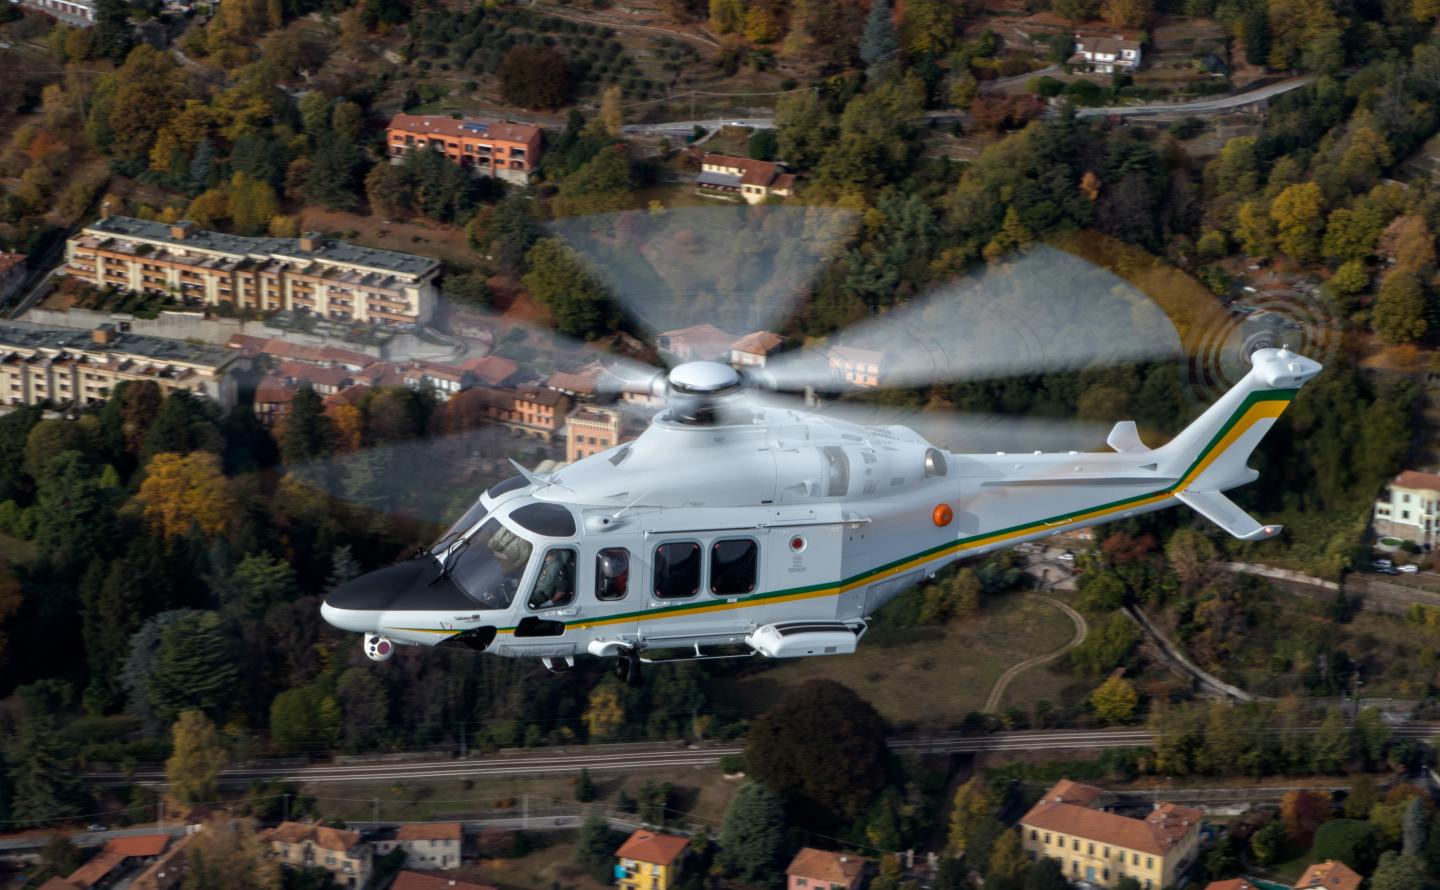
\includegraphics[width=0.5\textwidth]{Imagens/aw139.jpg}
    \caption{AgustaWestland AW139 Source:\cite{noauthor_undated-ue}}
    \label{fig:my_label}
\end{figure}
\FloatBarrier
Este helicópero apresenta as seguintes caracteristicas (Source:\cite{noauthor_undated-ue}):
\begin{table}[h]
\begin{tabular}{|l|l|}
\hline
Max Gross Weight                                                                                             & 6,400 kg 14,110 lb                                   \\ \hline
Increased Gross Weight                                                                                       & 6,800/7,000 kg 14,991/15,432 lb                      \\ \hline
Powerplant                                                                                                   & 2 x Pratt \& Whitney PT6C-67C Turboshafts with FADEC \\ \hline
Overall length (Rotors Turning)                                                                              & 16.66 m 54 ft 08 in                                  \\ \hline
Overall height (Rotors Turning)                                                                              & 4.98 m 16 ft 04 in                                   \\ \hline
Rotor diameter                                                                                               & 13.8 m 45 ft 03 in                                   \\ \hline
Capacity                                                                                                     & Crew 1-2 Passengers up to 15                         \\ \hline
Max Cruise Speed (ISA, MGW, SL, MCP)                                                                         & 305 km/h 165 kt                                      \\ \hline
HIGE (ISA, MGW, TOP)                                                                                         & 4,672 m 15,327 ft                                    \\ \hline
HOGE (ISA, MGW, TOP)                                                                                         & 2,476 m 8,123 ft                                     \\ \hline
\begin{tabular}[c]{@{}l@{}}Max Range (ISA, MGW, SL)\\ with auxiliary fuel tank - No reserve\end{tabular}     & 1,032 km 557 nm                                      \\ \hline
\begin{tabular}[c]{@{}l@{}}Max Endurance (ISA, MGW, SL)\\ with auxiliary fuel tank - No reserve\end{tabular} & 5 h 05 min                                           \\ \hline
\end{tabular}
\end{table}
\FloatBarrier
A massa máxima, bem como o \textit{max cruise speed} foram consideradas métricas importantes para comparar com o nosso design. 

%>>>>>
O nosso objeto era conseguir uma velocidade de cruzeiro superior com um veículo de menor massa, de forma a obter uma alternativa viável às soluções existentes.\par
% A velocidade de cruise deveria ser ultrapassada a fim de ser mais viável a nossa configuração e a massa deveria ser menor, conseguindo um design mais leve.\par
%<<<<<

A utilização duma powerplant igual à do AW139, constítuida por dois Turboshafts de 1 MW cada colocadas no topo da fuselagem \textbf{(citação??)} foi considerada para o nosso design como uma possibilidade (que acabou por ficar em todos as futuras iterações). 

%>>>>>
Apesar de neste ponto não ser considerada uma forma de propulsão em particular, foi considerado que caso se optasse por qualquer tipo de propulsão híbrida esta powerplant seria viável pois é uma configuração comum em helicópteros e a potência é semelhante à do XV-15, um tiltrotor de MTOW semelhante ao AW139 que também foi usado como referência na nossa pesquisa.\par
%Apesar de ainda, neste ponto, não se ter considerado uma arquitetura de propulsão, foi considerado que caso se optasse por uma turboeletrica ou com multiplos rotores e uma single power sorce, se poderia utilizar estas turbinas. Além de tal, foi considerada a sua posição, concluindo-se que se poderia utilizar a mesma localização, no topo da fuselagem, embedded.\par
%<<<<<

Além destes pormenores, a forma geral da fuselagem será parcialmente baseada no design do AW139.\par

\paragraph{Tilt Rotors and Tilt Wings}

%>>>>> refazer wording
No processo de geração de conceitos, procurou-se encontrar designs que seriam melhores que o helicóptero. Para tal, teve-se a ideia de que se poderia ter um cruise mais rápido e eficiente se se utiliza-se uma configuração parecida a um avião de asa fixa {\large{\textbf{Inserir citação or something sobre aviões serem melhores em cruise}}}. No entanto, sendo um avião e não um helicóptero, é necessário definir uma forma de ele realizar VTOL.\par
A pesquisa de configurações já existentes com estas qualidades resultou em ter em conta 3 aviões: XV-15, Bell Boeing V-22 Osprey, Bell V-280 Valor e LTV XC-142.\par
%<<<<< refazer wording 

O XV-15 foi um avião exprimental da NASA Tilt Rotor capaz tanto de descolagem vertical como voo horizontal, em modo de \textit{hover} ou \textit{cruise}.\cite{Maisel2001-fz} Estes modos estão apresentados na figura abaixo, aplicando-se em geral a tilt rotors.
\FloatBarrier
\begin{figure}[h]
    \centering
    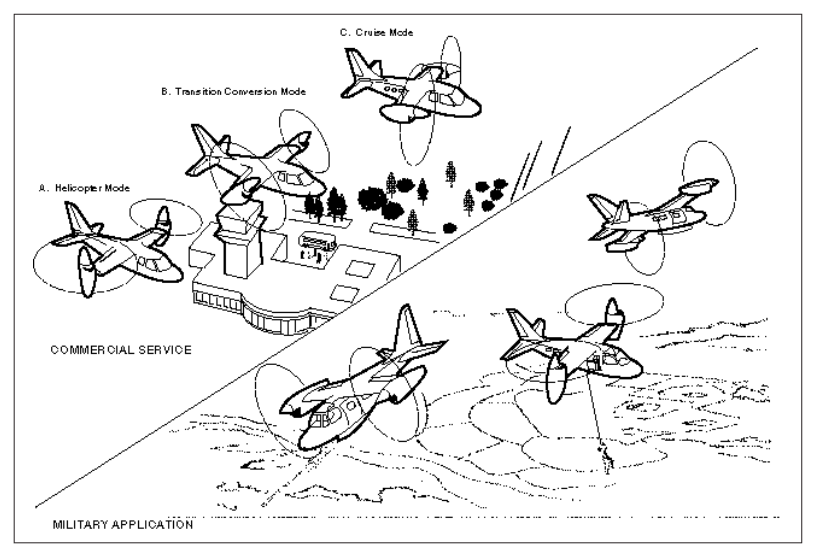
\includegraphics[width=0.7\textwidth]{Imagens/tiltrotor.PNG}
    \caption{"Illustration from 1974 Tilt Rotor Research Aircraft Project PlanSource":\cite{Maisel2001-fz}}
    \label{fig:my_label}
\end{figure}
\FloatBarrier
Dado estes modos de operação, bem como a capacidade de VTOL, este modelo impulsionou a solução de utilizar uma configuração tilt rotor no design. É apresentado, em baixo, o XV-15 a voar, de forma a enfatizar o facto de ser uma tecnologia testada que funciona. 

%>>>>>
Além de ter dois modos de voo, os rotores podem ser rodados para qualquer ângulo intermédio de modo a garantir eficiência máxima para todas as velocidades de voo.\cite{Maisel2001-fz}. 
%Além de tal, é importante referir que ele consegue voar com o "titl" intermédio, podendo escolher voar de forma mais eficiente a baixas velocidades.\cite{Maisel2001-fz}. 
%<<<<<

Tal funcionalidade também é tida em conta na escolha de usar um tilt rotor.\par 


\FloatBarrier
\begin{figure}[h]
    \centering
    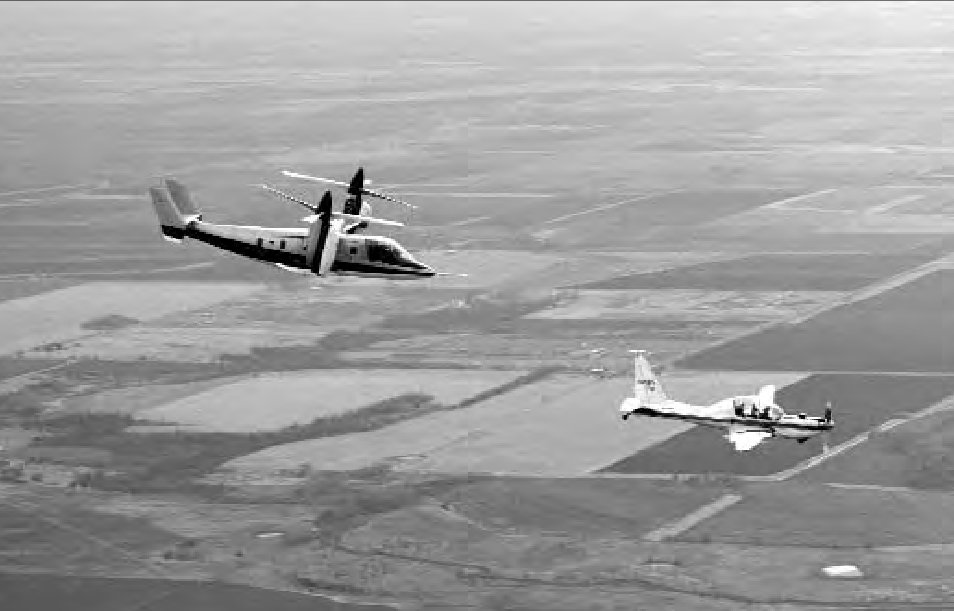
\includegraphics[width=0.5\textwidth]{Imagens/xv-15 cruise.PNG}
    \caption{"The XV-15 flying in close
formation with the YO-3A
for acoustics data.
(Ames Photograph
AC95-0438-15.1) Source:\cite{Maisel2001-fz}"}
    \label{fig:my_label}
\end{figure}
\FloatBarrier
O Bell Boeing V-22 Osprey é uma outra aeronave \textit{tilt rotor} considerada neste relatório. Neste caso, não é exprimental, sendo largamente utilizada, nomeadamente no contexto militar. Tal, mais uma vez, vem a viabilizar o tilt rotor como escolha possível.\par
{\large{\textbf{SOMEHOW É SUPOSTO MENCIONAR PERFIS DE VOO? Delille, completa, que tinhas dito isso}||| ze do que é que estas a falar what eu disse o que de que perfis de voo? tas a falar do facto de poder voar com angulos diferentes de tilt? like, ja mencionamos isso no xv15, dizemos so "tal como o xv15 o v22 tb faz angulos intermedios?? quais perfis de voo"}}\par
O Bell V-280 Valor, também uma aeronave tilt-rotor da Bell, criada como sucessor do V-22 com o objetivo de corrigir problemas no seu design original, é considerado como de importância devido ao uso de um "Non-Rotation Engine".\cite{noauthor_undated-gb}. Em baixo, de forma a ser mais claro, é apresentado a imagem de tanto a aeronave como desta informação, presente no site oficial da Bell.\par
\FloatBarrier
\begin{figure}[h]
    \centering
    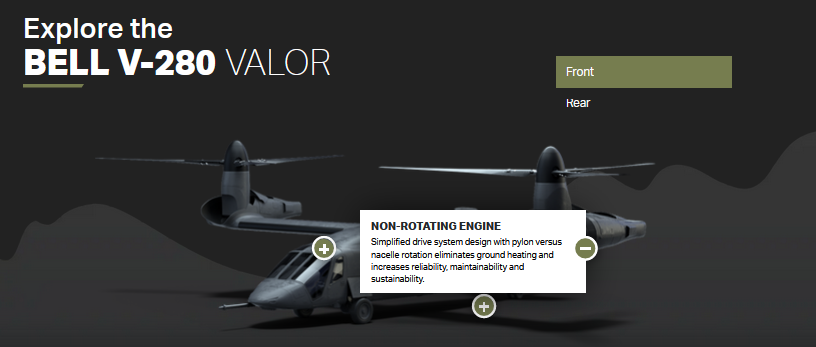
\includegraphics{Imagens/v_280.PNG}
    \caption{V-280 Source:\cite{noauthor_undated-gb}}
    \label{v-280}
\end{figure}
\FloatBarrier
Esta forma de girar os rotores de forma a se poder realizar VTOL, permite o uso de motores não só no centro das asas, o que não seria possivel se se rodasse a nacela do motor inteira. É de notar, no entanto, a interferência da asa com a esteira do rotor quando este está em posição vertical. Isto pode ser mitigado ao afastar o rotor da asa para permitir que a asa obstrua uma menor área do rotor.\par
O LTV XC-142 foi o único exemplo de uma aeronave de asa fixa VTOL encontrado durante a pesquisa que faz uso de \textit{tilt wings} em vez de \textit{tilt rotors}. {\Large{\textbf{Inserir citações, nomeadamente sobre como tilt wing é uma autentica complicação mecanica e tal}}}.\par
\subsection{Inicial Concept}
Inicialmente, foram realizados dois designs, em baixo apresentados.
\FloatBarrier
\begin{figure}[h]
    \centering
    \begin{subfigure}[b]{0.47\textwidth}
        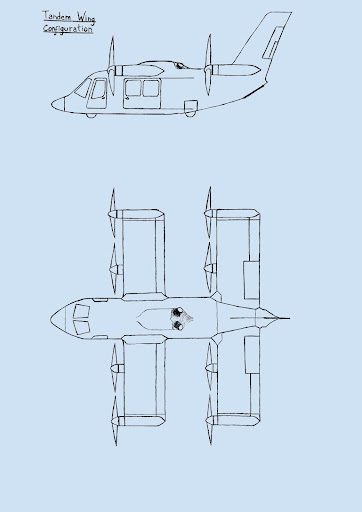
\includegraphics[width=\textwidth]{Imagens/inicialdesign1.jpg}
        \caption{Primeiro Design Sketch 1}
        \label{DesingSketchini1}
    \end{subfigure}
    \hfill
    \begin{subfigure}[b]{0.47\textwidth}
        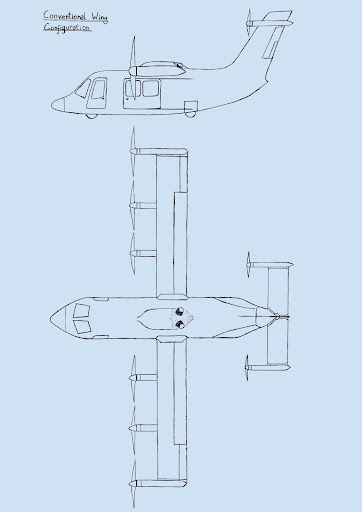
\includegraphics[width=\textwidth]{Imagens/inicialdesign2.jpg}
        \caption{Primeiro Design Sketch 2}
        \label{DesingSketchini2}
    \end{subfigure}
    \caption{Conceitos Iniciais - Semana 1}
\end{figure}
\FloatBarrier
Ambos os esboços apresentam uma fuselagem alongada, com um nariz semelhante ao AW139. No entanto, como não é necessário um rotor de cauda para controlar a guinada, em vez de ter uma cauda estreita e alongada foi escolhida uma cauda mais curta com maior volume interno semelhante a um avião convencional, na qual assenta o estabilizador horizontal. Apresentam, igualmente, uma porta lateral, como no AW139.\par
Notar que os desenhos são puramente qualitativos e não apresentam proporções ou posições exatas das várias partes. Tendo tal em conta, nota-se que as pás dos rotores da asa da figura \ref{DesingSketchini2} encontram-se em frente à porta, o que não deverá acontecer no design final.\par
Ambas as configurações, apesar de não estar explícito nos desenhos, deverão apresentar a configuração tilt rotor presente no Bell V-280.\par
O trem de aterragem é baseado no AW139, sendo triangular.\par
A grande diferença entre as duas configurações é o facto de a primeira ser Tandem Wing, enquanto que a segunda apresenta uma configuração convencional com a cauda em cruz. O estabilizador vertical é colocado acima da asa principal na figura\ref{DesingSketchini2} de forma a diminuir a interferência nesse mesmo por ela causada.\par
%>>>>>
A configuração \textit{tandem wing} é proposta como solução para o problema da restrição de tamanho imposta pelos heliportos, pois receávamos que para obter uma área de asa suficiente para sustentar a aeronave em voo cruzeiro esta teria de ter uma envergadura demasiado longa para caber dentro de um heliporto, ou teria de ter uma corda tão grande que não seria eficiente. Usando uma \textit{tandem wing} a área da asa é efetivamente duplicada mantendo a mesma corda e envergadura, no entanto é difícil de estimar o ganho de eficiênicia relativamente a simplesmente duplicar a corda.\par
Além disto, esta configuração combinada com preciso controlo eletrónico do impulso gerado por cada rotor permite um melhor controlo de atitude em \textit{hover} devido à maior distância entre os rotores e o centro de massa.\par
%A tandem wing é proposta devido à restrição de tamanho do heliporto, dado que não é possivel ter uma asa com alto aspect ratio e obter a mesma área que a conseguida com a tandem wing. Apesar de ser mais ineficiente em geral do que apenas uma asa com maior aspect ratio, dado que esse pode não ser possível, coloca-se a hipótese cuja validade só poderá ser averiguada em estudos posteriores a esta fase.\par
%Além disto, esta configuração também permite uma distribuição mais equilibrada durante o VTOL devido ao quadcopter.\par
%<<<<<
Nesta fase, considerou-se propulsão puramente turboelétrica em que um gerador alimenta os motores diretamente sem intermediários, não sendo menicionadas, por isso, baterias.\par